%2multibyte Version: 5.50.0.2960 CodePage: 1252
\documentclass[11pt]{article}
\usepackage[colorlinks,pdfpagelabels,pdfstartview=FitH,bookmarksopen=true,bookmarksnumbered=true,linkcolor=blue,plainpages=false,hypertexnames=false,citecolor=blue, urlcolor=blue]{hyperref}
\usepackage{amsfonts}
\usepackage{amsmath}
\usepackage{graphicx}
\usepackage{amssymb}
\usepackage{longtable}
\usepackage{authblk}
\usepackage{pdflscape}
\usepackage{rotating}
\usepackage[round]{natbib}
\usepackage{booktabs}
\usepackage[hmargin=1.15in,vmargin=1.15in]{geometry}
\usepackage{setspace}
\usepackage{chngcntr}
\usepackage{verbatim}
\usepackage{multirow}
%\usepackage{appendix}
\usepackage[title]{appendix}
\usepackage[gen]{eurosym}
\usepackage{comment}
\interfootnotelinepenalty=10000
\setcounter{MaxMatrixCols}{10}

\renewcommand{\floatpagefraction}{0.85}
\setstretch{1.25}
%\input{tcilatex}
\begin{document}
%\pagenumbering{gobble}
\pagenumbering{arabic}
\author[1]{Elena Bobeica, Matteo Ciccarelli, Isabel Vansteenkiste}
\affil[1]{European Central Bank}
\title{The link between labor cost and price inflation in the United States and the Euro Area\thanks{
\vspace{-1ex} \textit{We would like to thank Gonzalo Castex, Jordi Gali, Giorgio Primiceri, Juan Rubio-Ramirez, Frank Smets, Thomas Westermann, the seminar participants at the University of Maastricht, at Banque de France and at Bundesbank, and the participants of the XXII annual conference of the central bank of Chile: `Changing Inflation Dynamics, Evolving Monetary Policy' held in Santiago, Chile on 25-26 October 2018, for useful comments and suggestions on a preliminary version of this paper. The views expressed in this paper are of the authors only and do not necessarily reflect those of the European Central Bank or the Eurosystem.}}}
% \vspace{-1ex} \textit{This paper has been prepared for the XXII annual conference of the central bank of Chile: "Changing Inflation Dynamics, Evolving Monetary Policy." held in Santiago, Chile on 25-26 October 2018. We would like to thank Giorgio Primiceri, Juan Rubio Ramirez, Frank Smets and Thomas Westermann for useful comments and suggestions on a preliminary version of this paper. The views expressed in this paper are of the authors only and do not necessarily reflect those of the European Central Bank or the Eurosystem.}}}

\date{This version: \today. 
}
\maketitle

% \begin{abstract}
% \medskip
% \noindent \textbf{JEL Classification}: \\
% \noindent \textbf{Keywords}: 
% \end{abstract}
% \pagebreak
% \setcounter{page}{1}\pagenumbering{arabic}

\maketitle

\begin{abstract}
\medskip
This paper documents and compares the link between labor cost and price inflation in the United States the euro area. Our results show that the dynamic interaction is time-varying and depends on the state of the economy and on the shocks hitting the economy. Our results show that it is more likely that labor costs are passed on to price inflation with demand shocks than with supply shocks. However, the pass-through is systematically lower in periods of low inflation as compared to periods of high inflation. We find however that while the pass-through has remained broadly unchanged in the euro area (or has even marginally increased), it has declined substantially in the United States and is now close to zero. We argue that the different evolution in the market power of firms in the two areas may drive these diverging developments over time.\\
\\
\noindent \textbf{JEL Classification}: C32, E24, E31\\
\noindent \textbf{Keywords}: Inflation, pass-through, labor costs, structural VAR, United States 

\end{abstract}
\clearpage

\pagebreak
\begin{comment}
\section*{Non-technical summary}

XXX

\pagebreak
\end{comment}

\section{Introduction}
\label{Introduction}
A key policy question in the post-Great Recession period is whether labour costs (i.e. productivity adjusted wages) are still a useful gauge for inflation developments. It is intuitive to expect that as the labor market tightens, labor costs pick up and translate into higher prices. Labor costs constitute a substantial share of business expenses and hence could be an important element in a firm's pricing decisions. Theoretically, this perspective is rooted in the post Keynesian cost-push inflation view whereby wage increases in excess of productivity are seen as putting upward pressure on prices, and wages are the exogenous variable determining the future direction of inflation.


A number of policy makers on both sides of the Atlantic have recently explicitly referred to this cost-push view when discussing the inflation outlook. For instance, in the United States, \cite{Powell18} noted that \textit{if unemployment were to remain this low for this long, employers would be pushing up wages as they compete for scarce workers, and rising labor costs would feed into more rapid price inflation faced by consumers}. In the euro area, \cite{ECB2018} expresses similar views.\footnote{Similar references on the link between labour cost and price inflation developments were made in a Bank of England speech by the external MPC member Saunders (20/4/2018) who noted that “the Committee forecasts a gradual pickup in domestic cost growth that would help keep inflation slight above target two and three years ahead even as currency effects fade”. For the Bank of Japan, the Deputy Governor Iwata (31/1/2018) noted in a recent speech that “the inflation rate is projected to rise in line with wage increases”.}

Empirically, the idea that rising labor costs should lead to higher prices in the short to medium run is grounded in the developments in the 1970s when the so called wage-price spiral was seen as causing inflationary dynamics. A number of studies have however cast doubts whether wages systematically have an independent influence on prices over shorter horizons. Analyses based on in-sample Granger causality type of tests have yielded mixed conclusions,\footnote{For instance \cite{EmeryChang96},  \cite{Sbordone_02}, \cite{Bidder2015}, \cite{Hess_Schweitzer_2000}, \cite{Gordon_88} and \cite{Darrat1994}  all conclude that there is no causal link from labor cost to price inflation. The former three studies do however document that the link goes in the other direction whereas the latter three find also not causal link in either direction. \cite{Banerji2005} instead does find that labor cost inflation leads price inflation, but only at peaks, whereas it lags at troughs. Finally, \cite{Rissman1995} finds that only in manufacturing and trade services, wages granger cause inflation.} whilst studies focused on out-of-sample forecasting find it difficult to ascertain that wages add information to inflation forecasts.\footnote{(see for instance \cite{Stock_Watson_2008}, \cite{Knotek_Zaman_2014}). Overall, these studies have found that for out-of-sample forecasts, wages do not provide significant additional information beyond what can already be gleaned from other sources, including prices themselves (\cite{Bidder2015}). At the extreme, \cite{Stock_Watson_2008} even show that models using common wage measures may perform worse than their preferred benchmark without wages.} For the euro area, the more scant literature sheds a more positive picture on the link between labor cost and price inflation. 

Other studies argue that the link between labor cost and inflation has weakened in recent decades. Concretely, \cite{Knotek_Zaman_2014} shows how the correlation between wages and prices has decreased since the mid-80s while \cite{Hu_Toussaint-Comeau_2010} find that wage growth does not cause price inflation in the Granger causality sense, especially after the mid-80s.  Similarly, \cite{Peneva_Rudd_2017} show how the pass-through of labor cost growth to price inflation in the US has declined over the past several decades (to the point where it is currently close to zero). One explanation put forward has been the better anchoring of inflation expectations in recent years. Another one is that low levels of inflation changes the wage-price nexus because of downward wage rigidities (\cite{Daly_Hobijn_2014}). Such a view was also empirically uncovered by \cite{Mehra_2000} who finds that in periods of low inflation, wages do not help to predict inflation while it does in high inflationary environment.\footnote{\cite{Zanetti2007} found similar results using Swiss data.}

Most of the literature on the link between labor cost and price inflation has been US based. Analysis for the euro area would confirm the US findings, however does shed a more positive light on the link between labor cost and price inflation. Indeed, most euro area studies do find a statistically significant pass-through from labor cost growth to inflation and that labor cost does add information when trying to forecast inflation.\footnote{On the pass-through, see \cite{IMF18}. On forecasting, see \cite{Dees_Gunter_14} and \cite{JarocinskiMackowiak2017}. Finally, at the micro level, \cite{WDN2009} find that wage and price changes feed into each other. Around 40 percent of the firms surveyed acknowledge that there exists a relationship between wages and prices.}

These results are unsurprising when looking back at economic theory. %, which concludes that the link between labor costs and prices could run in either direction.
In fact, according to the new Keynesian models the correlation and lead-lag relationship between labor cost and price inflation can be expected to depend not only on the degree of the prevailing price and wage rigidities in the economy but also on the type of shock that hits the economy. As a result, we should in fact expect that the link between labor cost  and price inflation varies across time. 

In this paper, we argue that the link between labor cost and price inflation is both state and shock dependent. We focus on whether the link depends on the level of inflation and on whether the economy is hit by a supply or a demand shock. The idea that the relationship between variables is shock dependent is not new. It has already been more extensively explored in the exchange rate literature (see e.g. \cite{Forbes_2018}, \cite{Comunale_Kunovac_2017} and references therein), but also more recently in understanding the Phillips curve relationship (see \cite{Gali_Gambetti_19}). However, its relevance for the link between labor cost and price inflation has also already been suggested (see for instance \cite{Hahn_Gumiel_18} and \cite{BCV19}). This paper follows the methodology laid out in \cite{BCV19}, which studies the shock dependence of the the pass-through from labour costs to price inflation in the euro area. Concretely, we estimate the link between labor cost and price inflation in a VAR system setting TO UPDATE 

Our results show XXX

The remainder of the paper is organized as follows. Section \ref{Section:Data} presents the data. Section \ref{Section:simpleVAR} analyses the link in a VAR set up and considers to what extent the link has changed over time or depends on the level of price inflation. Section \ref{Section:SVAR} presents results based on a structural VAR model. Section \ref{Section:Conclusion} summarizes and concludes.


\section{A First Glance at the data}
\label{Section:Data}

There are a variety of ways to measure labor cost and inflation. In our analysis, we follow the approach of \cite{Peneva_Rudd_2017} for the US and of \cite{BCV19} for the euro area. As US inflation measure, we use the core PCE price index, that is the chain price index for market-based personal consumption expenditures excluding prices for energy and food at home. For the euro area, we use the GDP deflator. This is the series for which we have the most reliable information over a long period of time. This is particularly relevant for our analysis, as we wish to understand how the link between labor cost and price inflation has evolved over time, in particular since the 1970s. 

To measures labor costs, we rely on labor compensation series.\footnote{We focus in our analysis on compensation series. These differ from wages in that they include employer contributions for social insurance, pension contributions, and employer payments for health insurance and other fringe benefits.} For the euro area, we use compensation per employee. Alternative series, such as compensation per hour or hourly labor cost, are only available since 1995. For this reason, our preferred measure is compensation per employee. Moreover, we find that the correlation between our measure (i.e. compensation per employee) and the other measures is rather strong in their overlapping sample periods. For compensation per hour the correlation is on average above 0.8CHECK.When comparing our measure with Eurostat's labor cost index during overlapping periods, the average correlation is around 0.6CHECK. For the United States we use hourly compensation for the nonfarm business sector. In our robustness analysis, we also consider the employment cost index as a proxy for labor compensation. Both series are comprehensive measures of labor related production costs. The former is more comprehensive in that it also covers proprietors, self-employed workers and those with substantial discretion over their own pay. The latter measure has the advantage that it is a fixed-weight Laspeyres index, that corrects for the effects of shifts in employment between high-wage and low wage jobs. We use as preferred series the hourly compensation for the nonfarm business sector as this series is available since 1948. The employment cost index series is ony available since 1981. %As an index, it is therefore conceptually close to the CPI// The Employment Cost Index (ECI) measures the change in the cost of labor, free from the influence of employment  shifts among occupations and industries (see Bosworth and Perry, Brookings: productivity and real wages: is there a puzzle).


\begin{figure}[!htbp]
\begin{center}
\caption{Unit Labor Cost and Core PCE inflation, year on year \% change}\label{fig:yoy_inflation_LC}
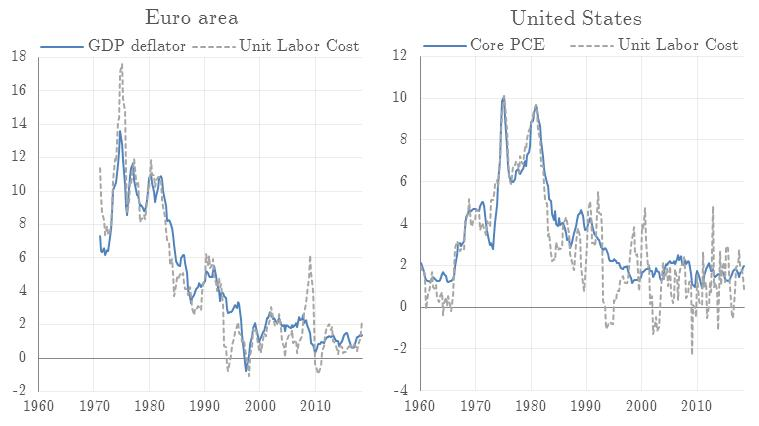
\includegraphics[scale = .95]{Chart_EAUS_data.jpg}
% trim={<left> <lower> <right> <upper>}
\begin{minipage}{0.92\textwidth} {\footnotesize
Sources: Authors' calculations.
Sample: 1960Q1-2018Q3.\par}
\end{minipage}
\end{center}
\end{figure}


To arrive at our labor cost measures, we subtract from both compensation series an estimate of the trend growth rate of average labor productivity.\footnote{For the euro area we use a measure of labor productivity for the economy as a whoe, for the US for the nonfarm business sector.} We prefer to subtract an estimate of \textit{trend} rather than actual productivity growth given that productivity growth is extremely noise at a quarterly frequency.\footnote{We compute the trend series in a similar manner as \cite{Peneva_Rudd_2017}. We compute a low pass filter on trend productivity growth in the same way as \cite{SSW01}, namely as the low-frequency component obtained from a band-pass filter of the annualized log difference of nonfarm business output per hour. We use an ARIMA(4,1,0) model to pad the actual productivity growth series prior to its 1947Q2 starting point; to pad the series after its 2018Q3 endpoint, we set the series equal to the CBO’s January 2018 forecast of average trend labor productivity growth from 2018Q4 to 2029 and to the 2029 value of the CBO forecast thereafter. The padded series is only used in the trend extraction routine, not to construct any of the unit labor cost series that we use in our VAR models.)}


\begin{figure}[!htbp]
\begin{center}
\caption{Adjusted unit Labor Cost and Core PCE inflation, year on year \% change}\label{fig:yoy_detrend_inflation_LC}
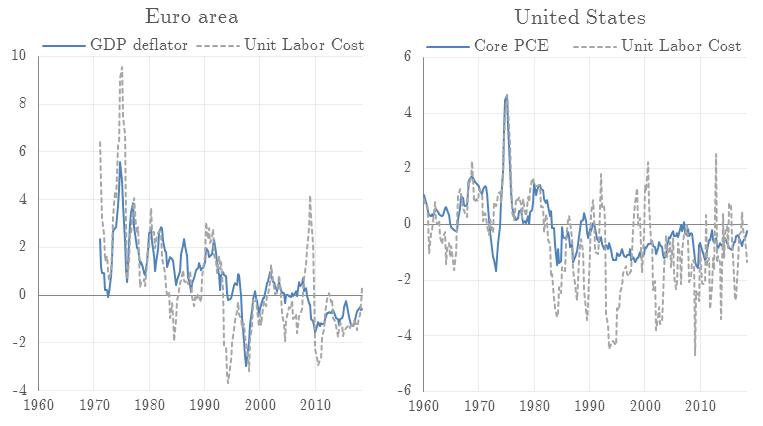
\includegraphics[scale = .95]{Chart_EAUS_datadetrend.jpg}
% trim={<left> <lower> <right> <upper>}
\begin{minipage}{0.92\textwidth} {\footnotesize
Sources: Authors' calculations.
Sample: 1960Q1-2018Q3.\par}
\end{minipage}
\end{center}
\end{figure}

Figure \ref{fig:yoy_inflation_LC} plots the year-on-year growth rate of our measures of labor cost and price inflation over the period 1960Q1-2018Q3 for the United States and 1971Q1-2018Q3 for the euro area. The high correlation between inflation and labor cost in both areas (0.94 for the euro area and 0.88 for the United States) demonstrates why policy makers continue to pay close attention to labor costs when assessing price inflation. In part the high co-movement between the two data series can be explained by a strong common (downward) trend over an important part of the sample (i.e. in the 1980s and early 1990s) which in turn can be attributed the improvements in the anchoring of inflation expectations towards lower levels. Given that this common movement is related to the improvements in the anchoring of inflation expectations to lower levels, we decided to adjust the series for a common movement. To do so, we follow \cite{Knotek_Zaman_2014} which is in turn inspired by the forecasting literature that has found gains in inflation forecasting accuracy by specifying inflation in gap form as the deviation from a slow-moving long-run trend (\cite{KozickiTinsley2001} and \cite{Zaman13}). Concretely, we construct labor cost and price inflation gaps by subtracting inflation expectations from the year-on-year growth rates of these series. As our preferred inflation expectation series is only available since 1979Q4 for the United States and from XXXCHECK for the euro area, we rely on an unobserved components model to create labor cost and price inflation gaps in the period prior to that. \footnote{The unobserved component model is estimated on the price inflation series and assumes that the inflation trend follows a random walk. This trend estimate from the unobserved component model is then applied to both the labor cost and price inflation series.}
The adjusted series are shown in Figure \ref{fig:yoy_detrend_inflation_LC}. This adjustment also implies that the series are stationary, according to a standard ADF unit root testCHECK.\footnote{CHECK:To ensure that our results do not depend on the approach taken, we also construct alternative price inflation and labor cost inflation gaps as year-on-year growth in these variables less a series-specific or shared long-run trend. Specifically we use an HP filter to adjust the series for the time span where inflation expectations were not available considered. The results in the paper were unchanged when applying this approach.}


\begin{figure}[!htbp]
\begin{center}
\caption{Scatter plot of Unadjusted (left pane) and adjusted (right pane) labor cost growth (6 months prior) and price inflation}\label{fig:Scatter}
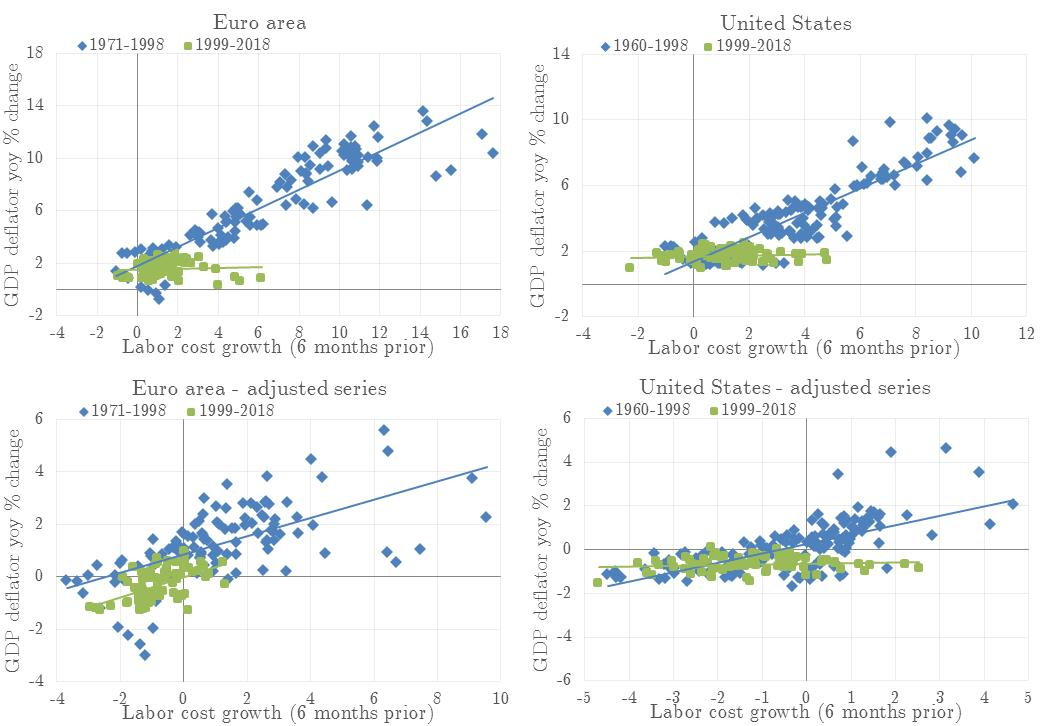
\includegraphics[scale = .75]{Chart_EAUS_scatter.jpg}
%trim={<left> <lower> <right> <upper>}

\begin{minipage}{0.92\textwidth} {\footnotesize
Sources: Authors' calculations.
Sample: 1981Q1-2018Q3.\par}
\end{minipage}
\end{center}
\end{figure}

The common trend is crucial in understanding the link between labor cost and price inflation. As shown in Figure \ref{fig:Scatter}, the correlation between price and labor cost inflation appear to have changed after the crisis when looking at unadjusted data, but there is no striking difference when considering the adjusted series. For the remainder of the paper, we will base our analysis on the adjusted series of labor cost and price inflation.


\section{A Simple VAR Analysis}
\label{Section:simpleVAR}

To examine in a dynamic and more conditional manner the link between labor cost and price inflation we estimate the relationship in a VAR setup. Our baseline VAR system contains three variables: the growth rates of (i) real GDP, (ii) labor cost and (iii) core PCE. The latter two variables have been adjusted as explained in Section \ref{Section:Data} to remove a common trend. The baseline estimation period ranges from 1961Q1 to 2018Q3 and is based on the employment cost index measure. The VAR system is estimated with four lags and Bayesian techniques assuming a normal-diffuse prior with a Minnesota prior on the matrix of coefficients to deal with the curse of dimensionality (see e.g. \cite{KadyialaKarlsson98}). UPDATE We also conduct a robustness check of our results by adding the spread between a long and a short-term interest rate to the VAR system. The included variable is intended to proxy for monetary policy.\footnote{UPDATE Our findings are largely unaffected by this extension, as shown in the Figures in Appendices \ref{AppendixCholeskiCountriesMP} and \ref{AppendixCholeskiCountriesHighLow_withMP}}

In this simple set up we can evaluate the impulse response function of core PCE inflation to a shock to ECI labor cost inflation by means of a Choleski orthogonalization with the variables ordered as listed above. The dynamic responses are used to answer the question: how much does price inflation rise when labor cost inflation rise by one-standard deviation. Standardized multipliers are computed mimicking the fiscal literature (see e.g. \cite{MountfordUhlig09}) as the ratio of the cumulative responses of price and labor cost inflation over the horizons 1 (impact) through 40 quarters. With such standardization, the multipliers are comparable across countries and sectors.

\subsection{Baseline estimation results}

We first report the estimated contemporaneous correlations between labor cost and price inflation computed from the moving average representation of the VARs (i.e. the impulse response estimates) truncated to 40 lags. 

Figure \ref{fig:CholeskiIRF_US} and Figure \ref{fig:CholeskiIRF_EA}, left pane plots the impulse response functions of price inflation to a shock to labor cost inflation, standardized as explained above in this Section. The estimates can be interpreted as pass-through multipliers from labor cost to price inflation. The middle and right pane of both Figures moreover show respectively the recursive and 30-year rolling window estimate of the long run (40 quarters ahead) pass-through coefficient.

\begin{figure}[!htbp]
\begin{center}
\caption{US: Choleski decomposition based pass-through from labor cost to price inflation}\label{fig:CholeskiIRF_US}
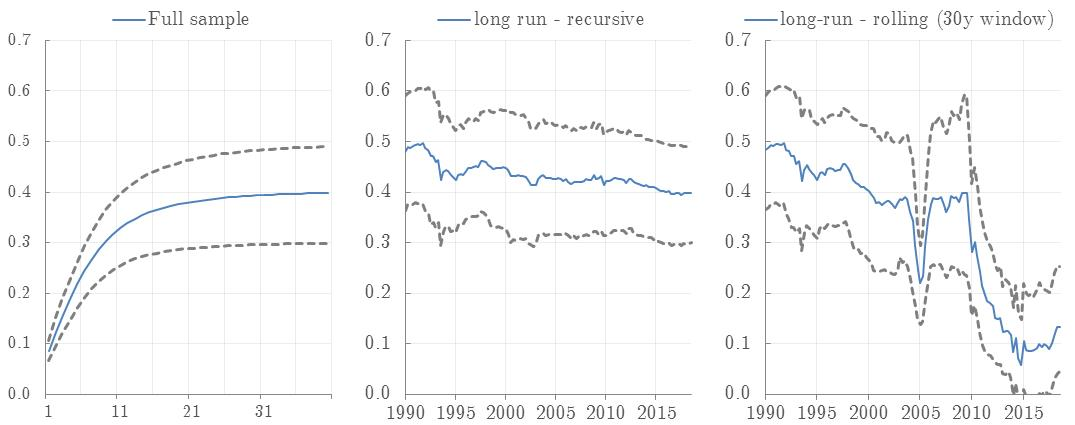
\includegraphics[scale = .7]{Chart_US_IRF_USEApaper.jpg}
% trim={<left> <lower> <right> <upper>}
\begin{minipage}{0.97\textwidth} {\footnotesize
Sources: Authors' calculations.\par}
\end{minipage}
\end{center}
\end{figure}


\begin{figure}[!htbp]
\begin{center}
\caption{EA: Choleski decomposition based pass-through from labor cost to price inflation}\label{fig:CholeskiIRF_EA}
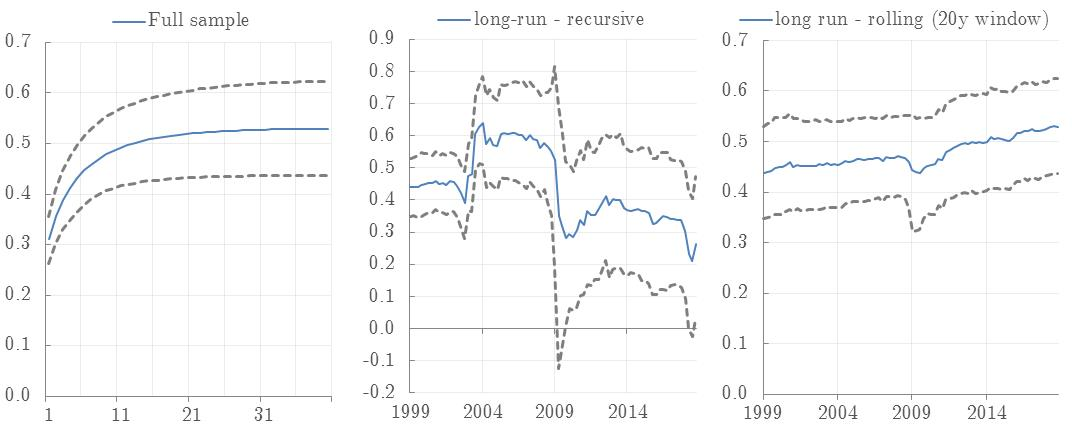
\includegraphics[scale = .7]{Chart_EA_IRF_USEApaper.jpg}
% trim={<left> <lower> <right> <upper>}
\begin{minipage}{0.97\textwidth} {\footnotesize
Sources: Authors' calculations.\par}
\end{minipage}
\end{center}
\end{figure}

These charts show that there is indeed a pass-through from labor cost to price inflation in both areas. Over the full sample, the pass-through coefficient is around 0.4 for the US and 0.53 for the euro area. Moreover, in line with other studies, we also find that the pass-through has been steadily declining over time in the United States and that this pass-through has been particularly low for the 30-year rolling windows that started in the mid-1980s and thereafter. By contrast, in the euro area, the pass-through has actually even increased over the rolling window sample.

% \pagebreak

% \textit{Implications for the behavior of the price-cost markup}

% From a theoretical perspective, the markup should be measured by the price-marginal cost fraction. Empirically, however, measuring the marginal cost is often fraught with important difficulties.\footnote{For a detailed discussion on the issues related to and existing approaches to measure the price-cost markup, see \cite{NekardaRamey13}.} For this reason, marginal cost is often proxied by average cost, and more precisely by average labor cost. Theoretically, a number of conditions exist under which the marginal cost equals the average cost. For instance with a Cobb-Douglas technology and no labor adjustment costs, the marginal wage would equal the average wage, and hence the price-average labor cost fraction would represent the markup. With a CES technology and perfect substitution of labour vis-a-vis other non-labour inputs it is also possible to show that the difference between price and labor cost inflation is the price-cost markup.
% Since we find an incomplete pass-through from labour costs to prices, our results have thus implications for the price-cost markup.\footnote{We acknowledge that other costs might make up part of the difference between price and labour costs growth, in particular the cost of capital. Nevertheless, grasping the cost of capital is a complicated problem beyond the scope of this paper and encompasses issues such as the price of intangible assets or quality-adjusted prices of information and communications technology goods.}  

% %a theoretical framework underpinned by Cobb-Douglas technology, no labor adjustment costs, and marginal wage equal to the average wage, the difference between price inflation and labor cost growth is equivalent to the change in the markup or profit margins. Since we find an incomplete pass-through from labour costs to prices, our results have implications for the behavior of profit margins.\footnote{We acknowledge that other costs might make up part of the difference between price and labour costs growth, in particular the cost of capital. Nevertheless, grasping the cost of capital is a complicated problem beyond the scope of this paper and encompasses issues such as the price of intangible assets or quality-adjusted prices of information and communications technology goods.}  



% % \begin{figure}[!htbp]
% % \begin{center}
% % \caption{Choleski decomposition based pass-through from labor cost to price-cost markup}\label{fig:Figure_CholeskiIRF_TotalEconomy_Margins}
% % \includegraphics[scale = .72]{Results_CholeskiIRF_TotalEconomy_Margins.jpg}
% % % trim={<left> <lower> <right> <upper>}
% % \begin{minipage}{\textwidth} {\footnotesize
% % Sources: Authors' calculations. The price-cost markup is calculated as the difference between the impulse response of price inflation to a shock to labor cost inflation.\par}
% % \end{minipage}
% % \end{center}
% % \end{figure}

% The implication from our estimation results for the price-cost markup is shown in Figure \ref{fig:Figure_CholeskiIRF_TotalEconomy_Margins} in Appendix \ref{AppendixCholeskiMargins}. The Figure shows the evolution of the price-cost markup as the difference between the impulse response of price inflation and labor cost inflation. Moreover, it also shows the cumulative response on the price-cost markup for the total economy. Overall, the Figure confirms, by looking at the results through a different lens, the incomplete pass-through with price-cost markups being squeezed following a positive labor cost shock.  Concretely, following a 1\% shock to labor cost inflation, the price-cost markup instantaneously declines in the total economy
% by around 0.8\% across countries.

\subsection{State-dependent pass-through: high versus low inflation}
Another important dimension in the context of the pass-through from labor cost to price inflation is to test the empirical proposition that this pass-through could depend on the level of price inflation. We look at this particular variable because reduced-form estimates of the pass-through from labor costs to price inflation capture the underlying nominal rigidities and the literature has highlighted that these rigidities may, inter alia, depend on the level of inflation. 

A low pass-through can be associated to a low inflation environment either because low inflation and low expected inflation persistence cause a low pass-through (\cite{Taylor00}), or because low levels of price inflation could be expected to reduce the pass-through due to downward wage rigidities (\cite{Daly_Hobijn_2014}). 
Another argument that has been suggested as to why the pass-through from costs to inflation could increase with the level of inflation is linked to the search intensity of consumers. Concretely, at low levels of inflation, a large fraction of buyers observe a single price. In that case, any given shock would increase price dispersion sharply, which would increase the search intensity of consumers, thereby reducing firm market power, which limits the ability of firms to pass on the cost increase to prices. At higher levels of inflation, price dispersion is higher and hence any given shock has only a limited impact on price dispersion and the search intensity of consumers. As a result, prices are at higher levels of inflation more responsive to shocks (see \cite{Head_10}). 

\begin{figure}[!htbp]
\begin{center}
\caption{Choleski decomposition based pass-through from labor cost to price inflation under low versus high price inflation}\label{fig:Choleski_highlow}
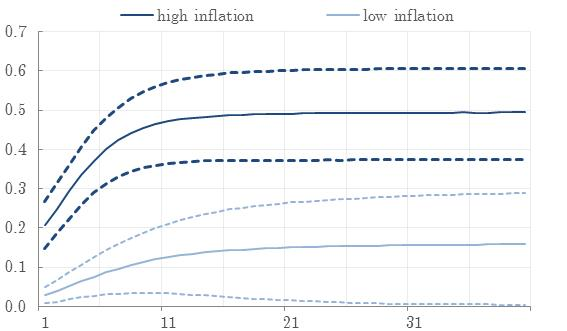
\includegraphics[scale = .85]{Results_US_CholskiIRF_highlowinfl.jpg}
% trim={<left> <lower> <right> <upper>}
\begin{minipage}{0.64\textwidth} {\footnotesize
Sources: Authors' calculations.\par}
\end{minipage}
\end{center}
\end{figure}

Finally, in a high-inflation environment profits might act less as a buffer than in a low-inflation regime due to an intertemporal smoothing of the profit path. For instance, when inflation is high and wages increase firms may expect an increase in interest rates which worsens their borrowing conditions and squeezes their future profit margins; hence, they will maintain their profits in the present, which would favor the pass-through from labor costs to prices. Conversely, the opposite might hold in a lower inflation regime where decreases in interest rates are expected. Another explanation could relate to the higher degree of economic uncertainty associated with a high inflation regime: in such a regime firms may simply not be prepared to buffer a labor cost increase with margins. Overall, the implicit margin responses in the high and low inflation regime, as shown in  Appendix \ref{AppendixCholeskiMarginsRegime_highlow}, confirm this intuition, i.e. that margins act less as a buffer under high compared to a low inflation regime.

Our sample is not long enough to test this proposition on two regimes. However, in our VAR analysis we can directly test this as the reduced-form estimates of the pass-through from labor costs to price inflation would capture the underlying nominal rigidities. Therefore, we repeat the above exercise by estimating the VAR over two sets of observations using a dummy variable approach, with the level of inflation in one subset being above and in the other being below the corresponding historical averages, respectively.Results are reported in Figure \ref{fig:Choleski_highlow}.

The findings support the theoretical and empirical literature. The pass-through from labor cost to price inflation is systematically higher if estimated over samples where the inflation rate is higher than the historical average. The finding also supports the view that a pickup in labor cost inflation is a necessary condition for rising inflation, to the extent that higher inflation expectations associated with a change from lower to higher inflation rates could raise the pass-through which in turn could speed up the inflationary process again.
\pagebreak


%%%%%%%%%%%%%%%%%%%%%%%%%%%%%%%%%%%%%%%%%%%%%%%%%%%%%%%%%%%%%%%%%%%%%
\section{The importance of underlying shocks in driving the pass-through from labor costs to inflation}
\label{Section:SVAR}

The previous section offered insights into whether labor costs are being transmitted to consumer price inflation, whether this link is visible when controlling for the business cycle and whether the link depends on the degree of nominal rigidities prevailing in the economy. This analysis, however, captures conditional correlations and does not allow us to identify the source of the correlation between labor cost and price movements; this is particularly important as this pass-through may be affected by various economic drivers acting simultaneously. In this section, we take a step further and argue that the pass-through is not a deep parameter underlying the economy, but depends on the structural shocks behind macroeconomic fluctuations.

Larger scale structural models trying to mimic the structure of the economy show that economic variables react differently to different shocks and the channels of transmission vary with each shock. Hence, also the relationship between variables is shock dependent. \cite{Gali_Smets_Wouters_12} make this point quite strongly in analyzing the relationship between unemployment and inflation; they show that a negative relationship is produced by demand shocks, whereas wage markup and supply shocks yield positive or near-zero comovement. 

In the same vein one can rationalize that the link between wage and price inflation is shock-dependent and depends on the degree of both price and labor cost stickiness following different shocks. The theoretical literature has focused so far on the impact of shocks on both labor cost and price inflation rather than on the pass-through of labor costs to price inflation following such shock. Given the puzzling behaviour of inflation in the aftermath of the Great recession, attempts have been made to dig deeper in the relationship between the two. Using one of the ECB's macroeconomic models, the New Area-Wide Model, \cite{Hahn_Gumiel_18} find that the response of the GDP deflator under demand shocks is qualitatively and quantitatively distinct from the response under supply shocks. The pass-through is stronger for demand than for supply shocks, with the key difference given by the behaviour of profit margins, which increase after a positive demand shocks (amplifying the pass-through from labor costs to prices). Also for the euro area, \cite{BCV19}, [Hahn,19?], [BdI] aim to translate such observations based on rich structural models to more tractable smaller scale models.\footnote{The idea of shock-dependent relationship between variables explored within an SVAR framwework has recently become prominent in the exchange rate empirical literature (see e.g. [cite the forthcoming ERPT taskforce OP], \cite{Forbes_2018}, \cite{Rincon-Castro_18}, \cite{Comunale_Kunovac_2017} and references therein), but also in understanding the Phillips curve relationship (see \cite{Gali_Gambetti_19}).} So far, we have not seen similar attempts for the case of the US, which is the focus of this paper.

%\cite{Bils_Chang_2000} did put forward a theoretical framework in which price rigidity differs with the nature of shocks, with prices being more responsive to increases in costs generated by factor prices than to an increase in marginal costs generated by an expansion of output. Model-based results show that prices react more to a technology (supply) shock than to a preference (demand) shock. Although this paper spells out clearly that it is important to disentangle between the nature of the shocks in seeing how prices react, it does not speak precisely to the question we are interested in, i.e. the pass-through from wages to prices.



%%%%%%%%%%%%%%%%%%%%%%%%%%%%%%%%%%%%%%%%%%%%%%%%%%%%%%%%%%%%%%%%%%%%%%%%%%
\subsection{A parsimonious structural VAR analysis}

We investigate the shock dependency of the pass-through from labor costs to inflation first in the most parsimonious set-up presented in Section X, by considering on top of the two nominal variables of interest a measure of economic activity. We identify a demand and a supply shock by imposing the classical restrictions of a positive co-movement between inflation and activity in case of demand shocks and a negative co-movement in case of supply shocks (see \ref{tab: identification1}). "A third shock in the model is left unidentified. The restrictions are imposed only for the first period and as inequality restrictions. The VAR is estimated as in the previous Section with Bayesian techniques and a normal-diffuse prior with a Minnesota prior for the mean and the variance of the VAR parameters. Impulse responses are computed based on 5000 draws from the posterior simulators." 

\begin{table}[!h]
\begin{center}
\caption{The 2 shock VAR: identification scheme}
\vskip 0.5cm
\label{tab: identification1}
%\resizebox{\textwidth}{!}{
\begin{tabular}{lccc}
\toprule
\textit{Variables} & \multicolumn{3}{c}{\textit{Shocks}} \\ \\[-1ex]
& Demand   & Supply  & Other \\
Real value added & \textbf{+} & \textbf{+} & $\bullet$ \\
Prices & \textbf{+} & \textbf{-} & $\bullet$ \\
Labor cost & $\bullet$     & $\bullet$     & $\bullet$ \\
\end{tabular}
\end{center}
\par
{\small \begin{center}Notes: $\bullet$ = unconstrained, \textbf{+} = positive sign,
\textbf{--} = negative sign \end{center}}
\end{table}

No restrictions were imposed for the path of labor costs, as a certain shock can affect wages and productivity in the same direction and the relative impact is not straightforward. Indeed, the results reported in \ref{AppendixSVAR} show that following a demand shock, labor costs tend to increase. The increase in wages outweighs that in productivity. The same goes for a supply shocks.   

Once the structural shocks underlying the economy have been identified, we first investigate the co-movement of price and labor cost inflation conditional on the structural shocks. This is done in the spirit of \cite{Gali_99} by constructing the counterfactual labor cost and price inflation that would be generated by a demand or a supply shock and check how the correlation structure between the counterfactual variables changes according to the shock. 

Figure \ref{fig:2ShockVAR_Correlation} reports the counterfactual labor cost inflation and price inflation that would have been generated by demand or supply shocks only based on the historical decomposition. One can see that demand shocks affect price and labor cost inflation in very similar ways. Supply shocks generate different patterns in the two nominal variables and labor cost appears to lead price inflation by [x] quarters. This result sheds new light on the results found by the previous literature, where there is no consensus on which variable leads which and results seemed very much sample dependent. We argue that similar to the lessons coming from the rich structural models, one would have to take into consideration the constellation of shocks driving economic developments to understand the link between prices and labor costs.

\begin{figure}
\begin{center}
\caption{Contribution of demand and of supply shocks to labor cost inflation and to core PCE}\label{fig:2ShockVAR_Correlation}
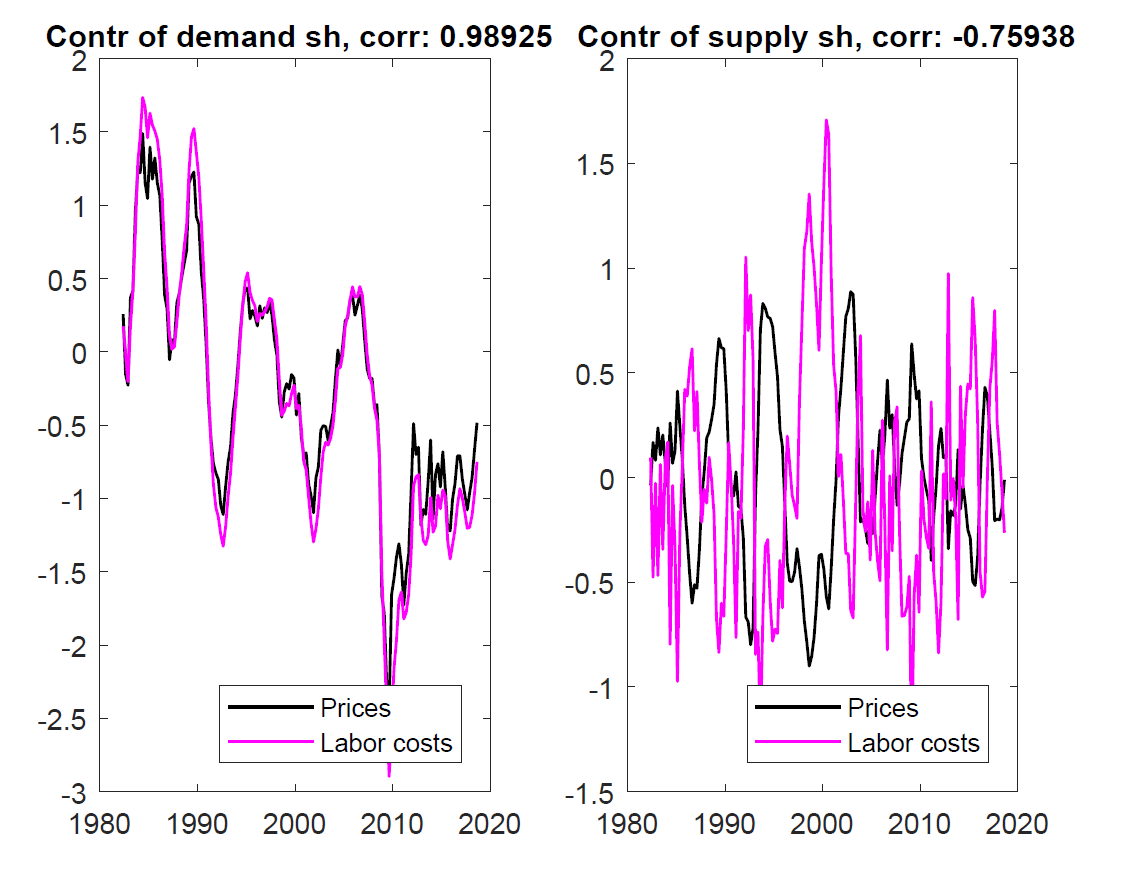
\includegraphics[scale = .5]{US_2shockVAR_Contrib.png}
% trim={<left> <lower> <right> <upper>}
\begin{minipage}{\textwidth} {\footnotesize
Note: ..
Sample period: 1960Q1-2018Q3.\par}
\end{minipage}
\end{center}
\end{figure}

In a second step we try to go beyond conditional correlations and check the shock-dependency of the pass-through from labor costs to inflation. We apply the methodology proposed in \cite{BCV19} to construct counterfactual scenarios in which we will check the response of price inflation to a certain shock assuming that the labor cost channel is shut down. The difference between the unrestricted inflation response and the counterfactual inflation response (assuming that labor cost inflation does not react) is an indication of the importance of the labor cost channel as an amplifier for the response of price inflation. 


"To give an intuition for this approach, consider a positive demand shock which boosts prices as firms have a higher pricing power and their demand for inputs of production also increases. Of all the mechanisms through which demand shocks affect prices, one particular channel relates to labor costs. We would like to isolate this channel by gauging the impact of demand shocks on prices through labor costs. We will compute an impulse response function ($IRF$) where the response of labor costs to a demand shock is zero and check the difference between the unrestricted $IRF$ for price inflation and the $IRF$ for the same variable when labor costs do not react to demand shocks. This difference is an indication of how much of the impact of demand shocks on inflation is driven by labor costs.

The idea of studying amplification mechanisms in a VAR by building a counterfactual scenario in which a certain variable does not react to a particular shock has been previously explored for other purposes. The impact of oil price shocks has been assessed via the reaction of inflation expectations (see \cite{Wong_2015}) or via the reaction of monetary policy (see \cite{Kilian_Lewis_2011} or \cite{Bernanke_Gertler_Watson_97}, who took inspiration from an early version of \cite{Sims_Zha_2006}). \cite{Bachmann_Sims_2012} apply the same methodology to isolate the role of confidence in the transmission of government spending shocks, while \cite{Ciccarelli_Maddaloni_Peydro_15} identify the effects of monetary policy shocks via the credit channel. What these papers have in common is that they operate with a VAR framework identified with contemporaneous zero restrictions. In a Choleski framework each variable has a corresponding shock; it is straightforward to shut down the $IRF$ of a variable by constructing a sequence of hypothetical shocks in that variable in a recursive manner, such that its $IRF$ is zero at all times. 

When we move away from the Choleski identification scheme to one based on sign restrictions, as we propose in this paper, things get more complicated. Let's say we want labor costs not to react to demand shocks; there is no \textit{labor cost shock} to offset the response of labor costs to demand shocks. One would have to make certain assumptions on which other shocks are doing the offsetting (i.e. is it the technology, other shocks or, our preferred version, a combination of all shocks hitting the economy). Appendix \ref{AppendixCountIRFsFormulas} shows how we derive the counterfactual $IRFs$."

The results are presented in Figure \ref{fig:2ShockVAR_Counter}. They suggest that when the economy is hit by demand shocks increases in labor costs are passed through to prices in a notable manner, whereas no such pass-through is detected under supply shocks. This holds over the entire period. Results starting the 80s confirm the results in the previous section of a diminished pass-through no notable pass-through can be detected anymore. Our intuition is that this stylised version of the structure of the economy, while useful, does not dig deep enough in the nature of the shocks that drive the economy. Particularly when it comes to supply shocks, this simple identification scheme is not able to disentangle between various types of shocks with opposing implications for the link between labor cost and price inflation. One can imagine three types of such shocks, all of them increasing output and reducing prices: (i) a positive technology/productivity shock, which increases wages; (ii) a negative wage mark-up shock, which reduces wages; and (iii) a positive labor supply shock, which also reduces wages. The next subsection puts forward a richer identification scheme.  

\begin{figure}[!h]
\begin{center}
\caption{Unrestricted and counterfactual IRFs in the 2
shock VAR}\label{fig:2ShockVAR_Counter}
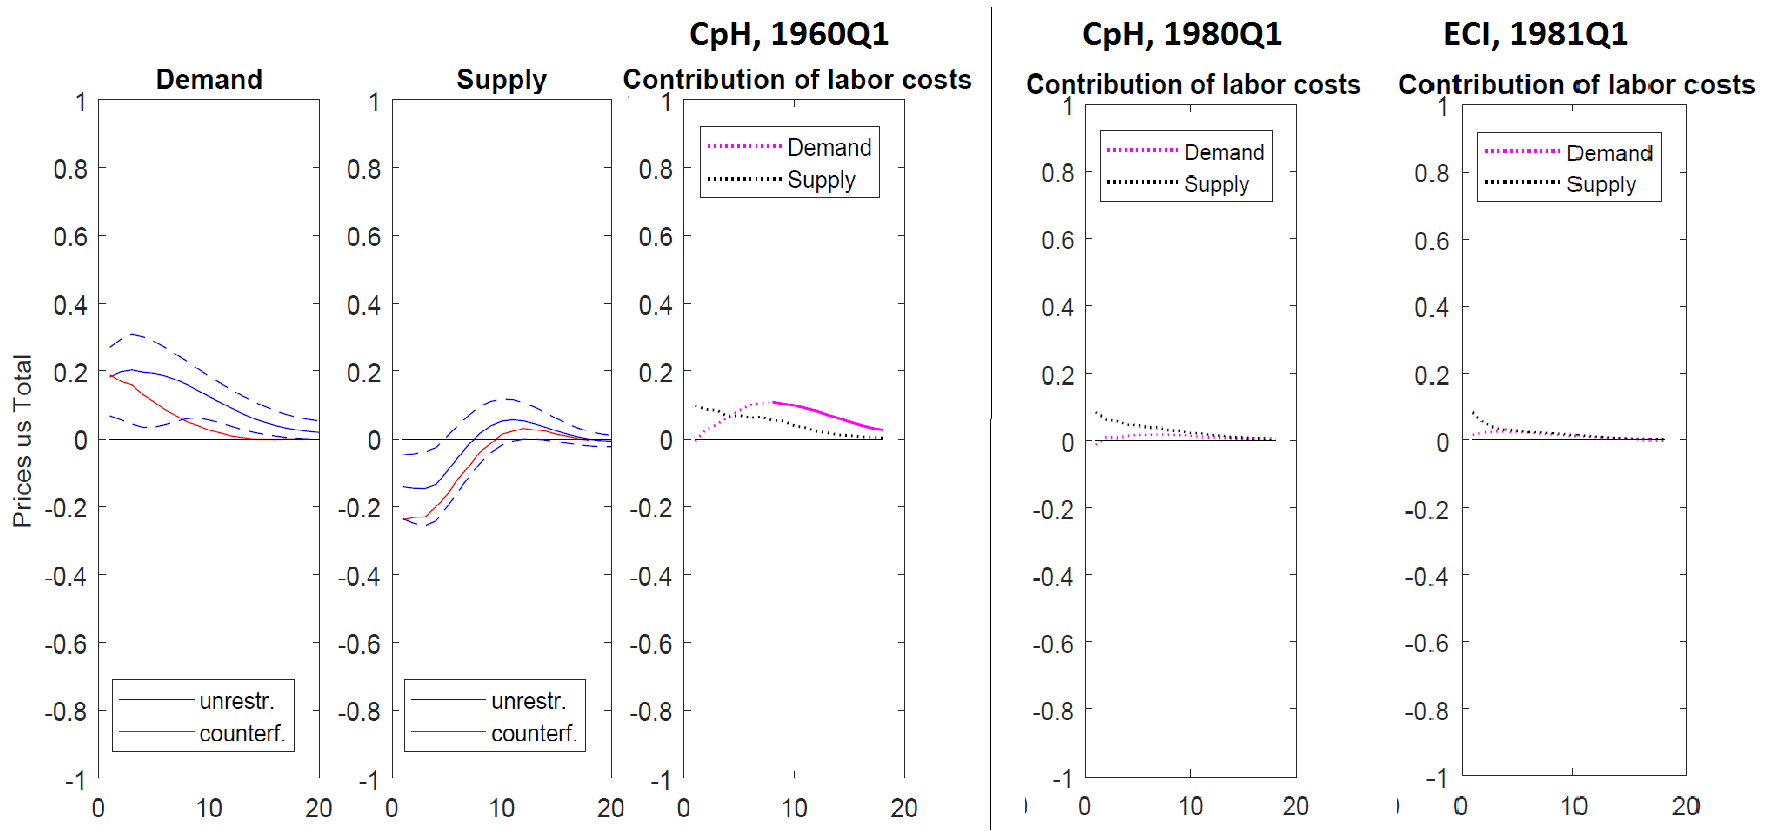
\includegraphics[scale=0.4]{US_2shockVAR_Counter_all.png}
% trim={<left> <lower> <right> <upper>}
\begin{minipage}{\textwidth} {\footnotesize
Note: The solid line in the third panel indicates the significance of the amplification channel.
Sample period: 1960Q1-2018Q3.\par}
\end{minipage}
\end{center}
\end{figure}


\subsection{A structural VAR with  labor market shocks and monetary policy}
%We put forward a VAR that covers shocks from the three  main categories: demand, labor market and supply.
In this subsection we aim to better model the structure of the economy by distinguishing 2 demand shocks: aggregate demand and monetary policy and 3 supply shocks: aggregate supply (technology), labor supply and wage mark-up shocks. In order to do that we have to separate labor cost inflation into its main components, wage and productivity growth. The restrictions are again imposed on impact and are spelled out in Table \ref{tab: identification2}. 


\begin{table}[!h]
\tiny
\begin{center}
\caption{The 5 shock VAR: identification scheme}
\vskip 0.5cm
\label{tab: identification2}
%\resizebox{\textwidth}{!}{
\begin{tabular}{lcccccc}
\toprule
\textit{Variables} & \multicolumn{3}{c}{\textit{Shocks}} \\ \\[-1ex]
& Demand   & Supply & Labor supply & Wage mark-up & Monetary pol & Other \\

Real value added & \textbf{+} & \textbf{+} & \textbf{+} & \textbf{+} & \textbf{+} & $\bullet$ \\
Prices & \textbf{+} & \textbf{-} & \textbf{-} & \textbf{-} & \textbf{+} & $\bullet$ \\
Wages & \textbf{+} & \textbf{+} & \textbf{-} & \textbf{-} & \textbf{+} & $\bullet$ \\
Productivity & \textbf{+} & \textbf{+} & $\bullet$ & $\bullet$ & $\bullet$ & $\bullet$ \\
Unemployment rate & \textbf{-} & $\bullet$ & \textbf{+} & \textbf{-} & \textbf{-} & $\bullet$ \\
Spread & \textbf{+} & $\bullet$ & $\bullet$ & $\bullet$ & \textbf{-} & $\bullet$ \\
\end{tabular}
\end{center}
\par
{\small \begin{center}Notes: $\bullet$ = unconstrained, \textbf{+} = positive sign,
\textbf{--} = negative sign \end{center}}
\end{table}

The VAR is now composed of 6 variables, namely: real value added, GDP deflator, nominal compensation per employee, labor productivity,  unemployment rate and a prxy for the shadow rate. All variables except the unemployment rate and the shadow rate are expressed in annual growth rates, with the GDP deflator and nominal compensation adjusted by long term expectations, as previously discussed. The system can only be estimated on the total economies since unemployment rate data does not exist at the sectoral level. 

Besides the $classical$ demand and supply shocks, this system allows us to identify two more labor market shocks, as shown in Table \ref{tab: identification4shock}. A positive labor supply would increase the labor force participation, which translates into a positive impact on output and on the unemployment rate. Wage growth falls, and so does inflation; the different wages response allows disentangling labor supply from technological shocks, as explained in \cite{Peersman_Straub_09}. A wage mark-up shock, or a wage bargaining shock, is a shock that allows firms to capture a larger share of the bargaining surplus, which contributes to lower marginal costs, wage growth and inflation. Output increases and the unemployment rate decreases, as detailed in \cite{Foroni_18}.\footnote{The estimation has been performed using the BEAR toolbox, see \cite{Dieppe_2016}.} 

Results are reported in Figure \ref{fig:Amplif5shock}. The counterfactual $IRFs$ are constructed by imposing that the difference in wage and productivity growth is shut down after a certain shock hits. This Figure shows in a synthetic manner the quarters when we find a notable difference between the impulse responses with and without the labor cost channel by marking these quarters with blue cells. The white diamond shows the quarter for which this amplification reaches its peak.

\begin{figure}[!h]
\begin{center}
\caption{The amplification channel via labour costs in different specifications}\label{fig:Amplif5shock}
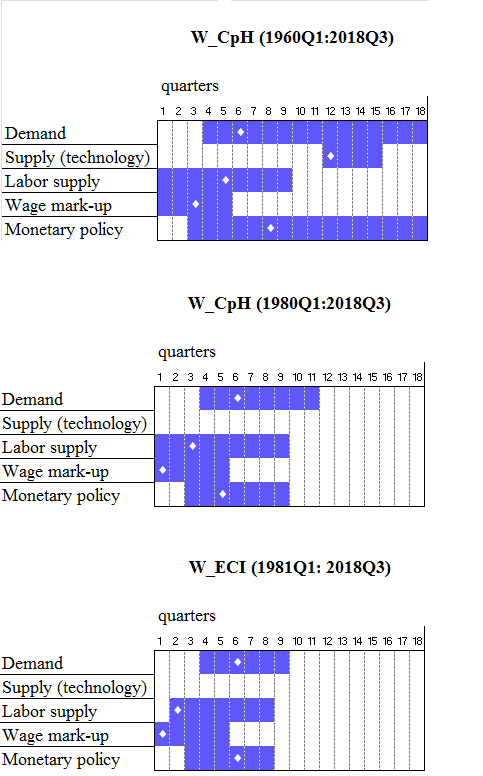
\includegraphics[scale = .8]{US_Amplif_5shock.png}
% trim={<left> <lower> <right> <upper>}
\begin{minipage}{\textwidth} {\footnotesize
Note: This chart indicates, in blue, the quarters following a demand or a supply shock where the median counterfactual IRF lies outside the 68 percent posterior uncertainty band of the unrestricted IRF; borderline cases were left out. The white diamond indicates the quarter for maximum impact of the price inflation response.\par}
\end{minipage}
\end{center}
\end{figure}


The results confirm our prior intuition. When digging deeper into the source of underlying shocks affecting the economy one can see that there is a significant pass-though from labor costs to price inflation even in the most recent period starting the 80s. This pass-through occurs under aggregate demand and monetary policy shocks and under labor market shocks; aggregate supply shocks do not seem to generate a robust pass-through of labor costs to inflation. It is worth noting that the peaks of this pass-through tend to occur at a higher lag for demand-type shocks than for supply-type shocks.


\subsection{Time variation in the pass-through and the shock constellation}

Figure \ref{fig:Histdec} suggests that the weaker co-movement between labor costs and price inflation observed in the data can be traced back to a changing composition of shocks hitting the US economy. In the most recent period, which has sparked the debate on whether such pass-through has vanished, the relative contribution of demand shocks has decreased, alongside with a slight increase in the contribution of monetary policy shocks and an increase in the relative contribution of supply shocks, for which the pass-through was found to be negligible. The contribution of wage mark-up and labour supply shocks appears to be relatively constant over time. 

\begin{figure}[!h]%[!htb]
\begin{center}
\begin{tabular}{ccc}
Historical decomposition &  & Rel importance of shocks \\
&  &  \\
%Simple benchmark: Choleski &  & Simple benchmark: Choleski \\
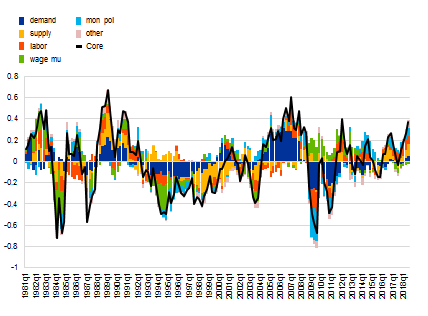
\includegraphics[width=0.50%
\textwidth]{US_HistDecPCE_80_CpH} &  & %
\includegraphics[width=0.50%
\textwidth]{US_Shocks_80_CpH} \\
\\
%Italy &  & Spain \\
%\includegraphics[width=0.50%
%\textwidth]{Margins_IT_Total} &  & %
%\includegraphics[width=0.50%
%\textwidth]{Margins_ES_Total} \\
%&  &
\end{tabular}
%\medskip
\parbox{1\textwidth}{\small The contribution of shocks in absolute value; moving average over 10 years - core PCE starting the 80s (SVAR with CpH).}\\
\caption{The changing relative importance of shocks}
\label{fig:Histdec}
\end{center}
\end{figure}


\subsection{Comparison with euro area}

In this sub-section we investigate to which degree the pattern of shock dependency uncovered for the US is valid also for the euro area. We apply the same 5 shock VAR and find very similar results (Figure \ref{EA_counter}). 


\begin{figure}[!h]
\begin{center}
\caption{The amplification channel via labour costs Under different shocks. GDP deflator, 1971Q1:2018Q3}\label{fig:EA_counter}
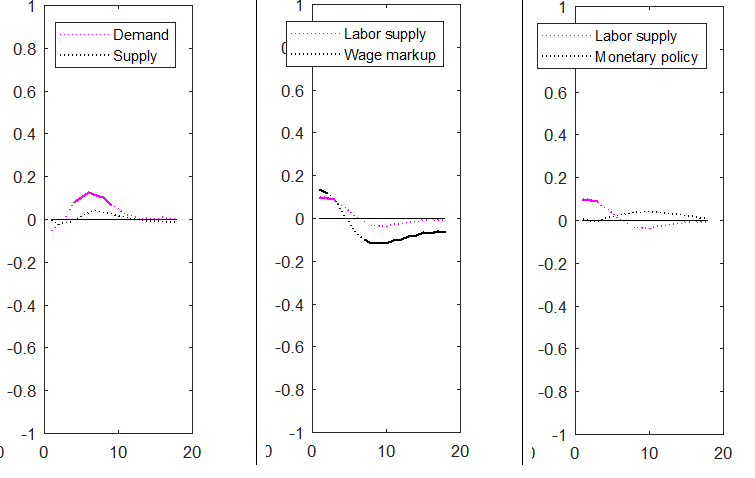
\includegraphics[scale = .8]{EA_5shockVAR_Counter.png}
% trim={<left> <lower> <right> <upper>}
\begin{minipage}{\textwidth} {\footnotesize
Note: ...\par}
\end{minipage}
\end{center}
\end{figure}





The question that arises from these results is: why would labor costs tend to be passed through to prices when the economy is hit by a demand rather than by a supply shock? 
%This analysis cannot provide a definite answer. But it can be reconciled with previous findings whereby the willingness of firms to increase prices after labor cost increases is larger when positive demand shocks dominate. In such an environment, the share of higher income consumers with lower demand elasticity increases, which in turn raises firms’ ability and power to pass-through cost increases to prices (see for instance \cite{Dornbusch_87} and \cite{Bergin_Feenstra_01}). This has implications for the differentiated behavior of the markup. In an environment where labour costs increase due to demand shocks, the price-cost markup would act as a buffer to a smaller extent than when the increase occurs due to supply shocks. The literature has stressed that the cyclicality of the markup is conditional on various types of shocks (see for instance \cite{GaliGertlerLopez2007} and \cite{NekardaRamey13}). We find that under a positive demand shock, margins are pro-cyclical (see Appendix \ref{AppendixMarginsSVAR2}). Initially the price-cost markup increases, as price inflation increases, while labor costs growth increases by less or even declines in some instances. In a second stage, margins start to decline, as labor cost growth starts to increase (e.g. employment increases with delay) and they subsequently stabilize. Under a positive supply shock, margins appear to be counter-cyclical. They decrease because price inflation falls, while labor costs growth increases. The evolution of the price-cost markup is similar in the unrestricted and counterfactual scenario. What differs is the magnitudes of adjustment. In the medium term, the price-cost markup tends to stabilize at lower levels in the unrestricted world compared to the counterfactual, which reflects a positive pass-through of labor costs to prices; also, this difference on the medium-term is more notable for the markup following a demand shock, which reflects the more sizable pass-through in case of demand shocks.     








The historical decomposition gives an intuition on the  the relative role played by the exogenous shocks at each point in time.

\section{Summary and conclusions}
\label{Section:Conclusion}
TO BE ADDED.

\pagebreak

\begin{appendices}
\section{Data documentation} \label{DataAnnex}
The inflation, labor cost and unemployment rate series were all obtained from the Bureau of Labor Statistics. Compensation per hour series are available since 1947Q1, whereas the Employment Cost Index is available since 1980Q3. Real GDP series are obtained from the Bureau of Economic Analysis (series in seasonally adjusted annual rates in 2012 billion chained dollars).

To proxy for the monetary policy stance, we use the effective Federal Funds rate. However, we use the shadow rate, as estimated by \cite{WuXia2016} over the period where the effective Federal Funds rate was at the \textit{zero lower bound}\footnote{Note that we define the period where the Federal Funds rate is at the zero lower bound any time in which the effective Federal Funds rate is in the 0 to 0.25 percent range targeted by the Federal Open Market Committee. Over our sample this was the case between end 2008 and end 2018.} .

Inflation expectations are difficult to measure. For the US, there exist a wide variety of approaches. As we wish to subtract from our inflation and labor cost series a slow moving low-pass trend from our series, we focus on long term inflation expectations. Ex ante it is unclear which long term inflation expectations measure would be preferable.  A number of measures are available: 
\begin{itemize}
\item Survey based inflation expectations – Michigan survey: Consumer survey for 5 year ahead inflation expectations. The series exist on a continuous basis since 1990Q4. (one year expectations available since 1978).

Additional information: http://www.sca.isr.umich.edu/
\item Survey based inflation expectations – Philadelphia Fed: 10-year ahead inflation expectations from survey among professional forecasters, available since 1991Q4.

Additional information: https://www.philadelphiafed.org/research-and-data/real-time-center/survey-of-professional-forecasters/
\item Survey based inflation expectations – Philadelphia Fed combined with historical data from other series: From 1991Q4 the 10-year ahead SPF inflation expectations are used. Prior to that, a combined series based on the Philadelphia Fed's Livingston Survey and from the Blue Chip Economic Indicators are used (information available back to 1979Q4). The gaps in the quarterly series are filled by means of a linear interpolation.

Additional information: https://www.philadelphiafed.org/-/media/research-and-data/real-time-center/survey-of-professional-forecasters/historical-data/additional-cpie10.xlsx?la=en 
\item Market based inflation expectations – computations by Groen and Middeldorp (2013): Breakeven backcast estimated 10 year inflation expectations as computed by Groen and Middeldorp.

Additional information: https://libertystreeteconomics.newyorkfed.org/2013/08/creating-a-history-of-us-inflation-expectations.html
\item Combined approach – computations by \cite{Cleveland12}: Methodology combines market and survey based inflation expectations. Inflation expectations are available for 1 to 30 years ahead. We chose the 10 year ahead series.

Additional information: https://www.clevelandfed.org/our-research/indicators-and-data/inflation-expectations.aspx
\end{itemize}

The various measures are shown in Figure \ref{fig:inflationexpectations}. We opt in our baseline analysis for the SPF survey based approach, combined with historical series from other sources, as provided by the Philadelphia Fed. 

\begin{figure}
\begin{center}
\caption{Measures of long-term inflation expectations \% change}\label{fig:inflationexpectations}
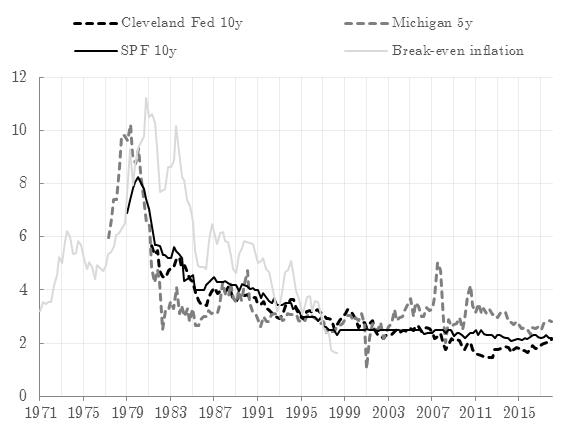
\includegraphics[scale = .75]{Chart_US_inflationexpectations.jpg}
% trim={<left> <lower> <right> <upper>}
\begin{minipage}{0.55\textwidth} {\footnotesize
Sources: Authors' calculations.
Sample: 1960Q1-2018Q3.\par}
\end{minipage}
\end{center}
\end{figure}

\clearpage

\end{appendices}


\clearpage

\newpage
\bibliographystyle{apalike}
\bibliography{passthrough_references.bib}
\end{document}
